% TEXINPUTS=.:$HOME/git/bvtex: latexmk  -pdf <main>.tex
\documentclass[xcolor=dvipsnames]{beamer}

\input{defaults}

\input{beamer/preamble}
\usepackage[outline]{contour}



\definecolor{bvtitlecolor}{rgb}{0.98, 0.92, 0.84}
\definecolor{bvoutline}{rgb}{0.1, 0.1, 0.1}

\renewcommand{\bvtit}{Wire Cell}
\renewcommand{\bvtitle}{\LARGE Wire Cell Software Overview \\
  (plus some data structure basics)}
\renewcommand{\bvevent}{BNLIF Wire Cell Team\\ 2015 April 2}
\renewcommand{\bvbeamerbackground}{}
\begin{document}
\input{beamer/title.tex}
\input{beamer/toc.tex}


\lstset{%
  language=C++,
                basicstyle=\scriptsize\ttfamily,
                keywordstyle=\color{blue}\ttfamily,
                stringstyle=\color{red}\ttfamily,
                commentstyle=\color{gray}\ttfamily,
                morecomment=[l][\color{magenta}]{\#}
}

\section{Source Code}

\begin{frame}
  \frametitle{Repositories}

  All our Wire Cell source code is in the ``BNLIF'' GitHub organization.

  \vspace{3mm}

  The main repository is:
  \begin{center}
    \url{https://github.com/BNLIF/wire-cell}
  \end{center}
  
  See full list or repositories at

  \begin{center}
    \url{https://github.com/BNLIF}    
  \end{center}

  \begin{itemize}
  \item Feel free to commit, make new ones, add issues, etc.
  \item Not all repositories in BNLIF are for Wire Cell.
  \end{itemize}
\end{frame}

\section{Names}

\begin{frame}[fragile]
  \tableofcontents[currentsection,hideothersubsections]
\end{frame}

\begin{frame}
  \frametitle{Package Names}

  A high-level naming convention is used:

  \begin{description}
  \item[source package] \texttt{wire-cell-<name>} used to name source repositories.
  \item[source subdir] \texttt{<name>} sub-directory location in a \textit{build
    package} of a \textit{source package} (more on this below).
  \item[binary package] \texttt{WireCell<Name>} used in expressing
    \textbf{dependencies} between packages and to name the public API
    \textbf{header directory}.
  \end{description}

  The source package/subdir names are somewhat unimportant but the
  \textbf{binary package name} gets baked to a few places.
\end{frame}

\begin{frame}
  \frametitle{Namespaces}

  C++ \texttt{namespace}s:
  \begin{description}
  \item[\texttt{units}]  the \textbf{system of units} taken from CLHEP \\
    (more on this next).
  \item[\texttt{WireCell}] all ``core'' C++ \textbf{library} code
    should be in this namespace.
    Don't add redundant ``WireCell'' name to class/function names
    themselves.
  \item[\texttt{WireCellXxx}] hold any code which \textbf{bridges}
    ``WireCell'' and some external code base.
  \end{description}

  Example of the last one: \texttt{WireCellSst} ``glues'' in the
  ``simple simulation tree'' (aka ``celltree'') data access.

\end{frame}

\begin{frame}[fragile]
  \frametitle{System of Units}

  \begin{lstlisting}
#include "WireCellData/Units.h"
int distance1 = 2.5*units::meter;
int distance2 = 10.0*units::meter;
cout << "The area is " 
     << distance1*distance2/units::centimeter2
     << " square centimeters" << endl;
  \end{lstlisting}
  Rules:
  \begin{enumerate}
  \item Do not ``care'' about a variable value's unit as long as it is
    in the \textbf{system of units}.
  \item Every \textbf{bare, literal} number should have a unit \textbf{multiplied}.
  \item To \textbf{express} a value in an explicit unit \textbf{divide} by the unit.
  \item If you \textbf{really really must} store an explicit unit in a
    variable the pick a variable name that implies the unit.
    (but, try to avoid this)
  \end{enumerate}
  \begin{lstlisting}
// avoid all these cases!
float energyCutMeV = 50; // bad, but at least name has unit
float angle_radians = some_angle / units::radian;
float pi_radians = 180.0*units::degree / units::radian;
\end{lstlisting}

\end{frame}

\section{Packages}

\begin{frame}[fragile]
  \tableofcontents[currentsection,hideothersubsections]
\end{frame}

\begin{frame}
  \frametitle{Source Package Types}

  Wire Cell has two basic source \textbf{package types}:
  \begin{description}
  \item[code] holds code for shared libraries, applications, tests,
    etc (most common)
  \item[build] includes one ore more code packages via ``\texttt{git
      submodule}'' method (just one now: \texttt{wire-cell})
  \end{description}

  You will mostly create and add to \textbf{code packages}.
\end{frame}

\begin{frame}[fragile]
  \frametitle{Code Package}
  \footnotesize
  \begin{itemize}
  \item A \textit{code package} holds the code to produce various build products.
  \item The build system assumes intent based on \textbf{layout conventions}:
  \end{itemize}
  \begin{description}
  \item[\texttt{src/}] source code (and private headers) for shared library
  \item[\texttt{inc/WireCellName/}]  public headers for shared library
    API.
  \item[\texttt{dict/LinkDef.h}] export API to ROOT dictionary.
  \item[\texttt{tests/}] unit tests (more on these below)
  \item[\texttt{apps/}] main programs, one \texttt{*.cxx} per app.
  \item[\texttt{python/WireCell/<Name>}] python modules (not yet
    supported in build)
  \item[\texttt{wscript\_build}] simple file hooking into the build system.
  \end{description}

  \vspace{1mm}

  Entire package build file is one line (\texttt{examples/wscript\_build})
  \begin{lstlisting}{language=Python}
bld.make_package("WireCellExamples", 
    use="WireCellNav WireCellData WireCellTiling WireCellSst")
  \end{lstlisting}
\end{frame}

\begin{frame}
  \frametitle{Current Packages}
  \footnotesize
  Roughly in order of increasing dependency:
  \begin{description}
  \item[\href{https://github.com/BNLIF/wire-cell-data}{\texttt{data}}]
    common \textbf{data classes}.
  \item[\href{https://github.com/BNLIF/wire-cell-nav}{\texttt{nav}}]
    data \textbf{navigation} (geometry, frames (``events'') and time slices)
  \item[\href{https://github.com/BNLIF/wire-cell-sst}{\texttt{sst}}]
    provides frame and geometry data source classes for \textbf{``simple
    simulation tree''} (aka ``celltree'') and accompanying wire
    geometry.
  \item[\href{https://github.com/BNLIF/wire-cell-tiling}{\texttt{tiling}}]
    things that produce or modify a \textbf{cell tiling}, includes 
    initial, reference implementation based on
    Michael's \texttt{CellMaker} (also available in that packages as an application.
  \item[\href{https://github.com/BNLIF/wire-cell-examples}{\texttt{examples}}]
    a growing set of \textbf{example} applications, python code, etc.
    Useful source of starting points.
  \item[\href{https://github.com/BNLIF/wire-cell-matrix}{\texttt{matrix}}]
    Xin's nascent area.    
  \item[\href{https://github.com/BNLIF/wire-cell}{(top)}] top
    level directory, source code aggregation, doxygen, and build
    package.
    (the \texttt{wire-cell} source package)
  \end{description}

  
  (labels are source subdirectory names)
\end{frame}

\section{Tests}

\begin{frame}[fragile]
  \tableofcontents[currentsection,hideothersubsections]
\end{frame}

\begin{frame}
  \frametitle{Tests Overview}
  \footnotesize
  Let's write well tested code!

  \vspace{2mm}

  \begin{itemize}
  \item You \textbf{already} write little tests when you write code 
    \begin{itemize}  \footnotesize
    \item (unless you are superman).
    \end{itemize}
  \item So, write them in a \textbf{useful form} from the start and
    keep them around:
    \begin{itemize}  \footnotesize
    \item Gives lots of examples how to use the code.
    \item Makes it safer to attempt needed changes to your code or others.
    \item Running tests can be (and is) automated so you can write
      once and then forget about them (until they fail)
    \end{itemize}
  \item One challenge: tests take \textbf{no arguments}
    \begin{itemize}   \footnotesize
    \item need to run same everywhere so no outside info
    \item leads to needing to mock up some things which can take extra effort
    \item if too hard, then write an \textbf{application} to hold your
      test and write instructions how to exercise it.
    \end{itemize}
  \item You can write tests in C++ or Python or Shell.
  \end{itemize}

  \vspace{2mm}
  \textbf{No excuses, write tests!}
  \Smiley[1.5]{}
  
\end{frame}

\begin{frame}
  \frametitle{Guidelines for Writing Useful Tests}
  \begin{itemize}
  \item Write \textbf{many, small} tests:
    \begin{itemize}
    \item Make each test just one thing.
    \item Limit the time any one test takes to run.
    \item Strive for complete testing coverage of your package.
    \end{itemize}
  \item Don't worry about test-code quality, \textbf{quick-and-dirty is better
    than non-existent}.
  \item Be conscious of \textbf{dependencies}
    \begin{itemize}
    \item don't let test code determine package dependencies
    \item make a new package just for tests if needed
    \end{itemize}
  \end{itemize}

  \vspace{3mm}

  It is better to write tests than to follow guidelines!
\end{frame}

\begin{frame}[fragile]
  \frametitle{C++ Tests}
  \begin{itemize}
  \item Mini application but no command line arguments allowed.
  \item Place code in \texttt{tests/test\_*.cxx}
  \item Auto-(re)built and (re)run as needed, not installed.
  \end{itemize}
  \begin{lstlisting}
// test_fail.cxx
int main(/*empty!*/) {
  exit(1); // 
}

// test_succeed.cxx
int main(/*empty!*/) {
  return 0;
}
  \end{lstlisting}

\end{frame}

\begin{frame}[fragile]
  \frametitle{Python tests}
  \begin{itemize}
  \item Form of one or more unit test \textbf{functions} per Python file.
  \item Place code in \texttt{tests/test\_*.py}
  \item Follow naming and the no-argument calling convention
  \item Automated running not yet added to build system
  \end{itemize}
  
 \begin{lstlisting}{language=Python}
# tests/test_fail_succed.py

def test_fail():     # name starts with test_ 
  "A test that always fails."
  raise RuntimeError

def test_succeed():  # function takes no args
  "A test that always succeeds."
  return
 \end{lstlisting}

\end{frame}

\begin{frame}[fragile]
  \frametitle{Shell tests}
  \begin{itemize}
  \item Form of an open-ended \textbf{shell script}, no cmd line arguments
  \item Run package's application(s) or those from other packages on
    which the package depends.
  \item Place code in \texttt{tests/test\_*.sh}
  \item Automated running not yet added to build system
  \end{itemize}
  
 \begin{lstlisting}{language=Shell}
#!/bin/bash
set -e         # fail early, fail often!
wd=$(mktemp -d)
cd $wd 
wget https://raw.githubusercontent.com/BNLIF/wire-cell-event/master/geometry/ChannelWireGeometry.txt
sst-geom-dumper ChannelWireGeometry.txt
rm -rf $wd    # clean up
 \end{lstlisting}
%$
 \footnotesize
 Note: we need to deal better with auxiliary data files and not rely
 on downloads from GitHub like this example.
 Maybe start depending on SQLite3 for simple database features.

\end{frame}


\section{Build}

\begin{frame}[fragile]
  \tableofcontents[currentsection,hideothersubsections]
\end{frame}

\begin{frame}
  \frametitle{Installation Overview}
  \begin{enumerate}
  \item Provide \textbf{external packages} (mostly ROOT\textbf{6})
    \begin{itemize}
    \item Automated externals installation method provided or,
    \item You are free to DIY
    \end{itemize}
  \item Set up your \textbf{run-time environment}.
    \begin{itemize}
    \item Automated installation provides two strategies
    \item DIY'ers must continue to DIY
    \end{itemize}
  \item Build \textbf{Wire Cell code} itself (details next)
  \end{enumerate}


  Note: automated \textbf{externals installation} method details here:
  \begin{center}
    \url{https://github.com/BNLIF/wire-cell-externals}    
  \end{center}
\end{frame}

\begin{frame}[fragile]
  \frametitle{Building Wire Cell}

  Prepare the source area
  \begin{lstlisting}{language=shell}
git clone git@github.com:BNLIF/wire-cell.git
cd wire-cell
git submodule init
git submodule update
alias waf=`pwd`/waf-tools/waf    
  \end{lstlisting}

Configure, build and install:
  \begin{lstlisting}{language=shell}
waf --prefix=/path/to/install configure build install
  \end{lstlisting}

Some developer dancing:

  \begin{lstlisting}{language=shell}
waf clean build  # force a full rebuild
waf              # rebuild after an edit
waf install      # (re)install 
  \end{lstlisting}


  More details in the
  \href{https://github.com/BNLIF/wire-cell}{wire-cell} source package
  README file.

\end{frame}



\section{Documentation}

\begin{frame}[fragile]
  \tableofcontents[currentsection,hideothersubsections]
\end{frame}

\begin{frame}[fragile]
  \frametitle{Documentation}
  \begin{itemize}
  \item Every package has a \texttt{README.org} file
    \begin{itemize}
    \item Simple text markup (\href{http://orgmode.org}{Org-mode})
      that GitHub renders.
    \item (note: there is \textbf{much} more to org-mode)
    \end{itemize}
  \item Code is peppered with Doxygen markup
    \begin{itemize}
    \item Optional: install \textbf{GraphVis} to get ``\texttt{dot}'' for nice graphs.
    \item TODO: I will add the running of Doxygen to the build
    \item TODO: Put Doxygen output on the web somewhere
    \item TODO: Got through source and add more doc strings.
    \end{itemize}
  \end{itemize}
  For now, run doxygen yourself:
\begin{verbatim}
$ doxygen docs/Doxyfile
$ firefox doxy/html/index.html
\end{verbatim}

  \begin{center}
    (\href{http://lycastus.phy.bnl.gov/~bviren/wire-cell-doxy/}{BNL internal link to doxygen})
  \end{center}
\end{frame}

\section{Tour of Wire Cell}

\begin{frame}[fragile]
  \tableofcontents[currentsection,hideothersubsections]
\end{frame}

\begin{frame}
  \frametitle{Basic Wire and Cell}
  Wire
  \begin{description}
  \item[Wire] geometry and numbering of one wire \textbf{segment}
  \item[WireSet] an owning collection of wires
  \item[WireSelection] a non-owning sub-set
  \end{description}
  Cell
  \begin{description}
  \item[Cell] geometry and numbering of one cell.
  \item[CellSet] an owning collection of cells
  \item[CellSelection] and non-owning sub-set
  \end{description}

  \texttt{Wire} and \texttt{Cell} objects are \textbf{static}
  information related to the detector and do not hold any dynamic
  (DAQ) data.
\end{frame}

\begin{frame}
  \frametitle{Charge and Time}
  \begin{description}
  \item[Trace] a starting \textbf{time} bin and a sequence of following \textbf{charges}
    from an electronics \textbf{channel}.
  \item[TraceCollection] A sequence of Trace objects
  \item[Frame] a \textbf{TraceCollection} with an \textbf{index} into the external
    ``frame data source'' (see nav below)
  \item[Slice] \textbf{[wire ID, charge]} pairs in same time bin across a
    \texttt{Frame} - this is what we reconstruction into Cells!
  \end{description}

  \footnotesize
  \begin{itemize}
  \item One full channel readout (eg, MB's 9600 time bins) can be
    represented by multiple \texttt{Trace} objects to allow for
    zero-suppression / analysis thresholds.
  \item A \texttt{Frame} object effectively corresponds to an ``event''
    (bad word!) with the \texttt{index} being the ROOT TTree entry.
  \end{itemize}
\end{frame}


\begin{frame}
  \frametitle{WireCellNav(igation)}
  \begin{description}
  \item[GDS] \texttt{GeomDataSource} gives information about the wire (segments) in the
    detector used to produce (and own) \texttt{Wire} objects.
  \item[FDS] \texttt{FrameDataSource} provides \texttt{Frame} objects, expect to
    write one FDS per data source type.
    \begin{itemize}
    \item WireCellSst/FrameDataSource is so far only one
    \end{itemize}
  \item[SDS] \texttt{SliceDataSource} takes any \texttt{FrameDataSource} and
    produces slices
    \begin{itemize}
    \item One SliceDataSource covers all needs.
    \item Requires a GDS to resolve channel $\rightarrow$ wire IDs
    \end{itemize}
  \end{description}
  Top-level user code will interact with all three of these objects.
  See \texttt{wire-cell-example-loop} for working example.
\end{frame}

\begin{frame}[fragile]
  \frametitle{Tiling}

  A tiling is a class which \textbf{creates and owns cells} and provides access to
  them and answers \textbf{queries} about their associations with wires.

  \vspace{2mm}

  Tilings inherit from \texttt{TilingBase} and must provide:

  \begin{lstlisting}
/// Must return all wires associated with the given cell
WireCell::WireSelection wires(const WireCell::Cell& cell) const;
        
/// Must return all cells associated with the given wire
WireCell::CellSelection cells(const WireCell::Wire& wire) const;

/// Must the one cell associated with the collection of wires or 0.
WireCell::Cell* cell(const WireCell::WireSelection& wires) const;
  \end{lstlisting}

\end{frame}

\begin{frame}
  \frametitle{Types of tilings}

  Tilings we have or will soon have$^*$:
  \begin{description}
  \item[TileMaker] the cell making code from Michael's CellMaker
  \item[TriangleTiling$^*$] special purpose exploiting MB's symmetry
  \item[Filter tilings$^*$] tilings that take other tilings as input,
    mostly to reduce available cells based on:
    \begin{itemize}
    \item removing chargeless wires
    \item ranking of cells
    \item info from a cell in neighboring slices
    \item kinematic fitters
    \end{itemize}
  \end{description}
  Tilings are nodes to construct high-level process flows:
  \begin{itemize}
  \item chain individual tilings to produce final result
  \item supports branches, iterations, recombinations
  \end{itemize}

\end{frame}


\section{Container Data Structures (for Xin)}

\begin{frame}[fragile]
  \tableofcontents[currentsection,hideothersubsections]
\end{frame}

\begin{frame}[fragile]
  \frametitle{Vector}

  Used best for collections where order is determined at fill time.
  \begin{itemize}
  \item ``Array'' type behavior
  \item Cheap random access, expensive insertion
  \end{itemize}

  \lstinputlisting{test_vector.cxx}

\end{frame}

\begin{frame}[fragile]
  \frametitle{List}

  Used best for collections where order may be determined later
  \begin{itemize}
  \item ``Doubly linked list'' behavior
  \item Cheap insertion, no random access ($\mathcal{O}(N)$)
  \item Reverse iteration, insertion, erasure
  \end{itemize}

  \lstinputlisting{test_list.cxx}
\end{frame}

\begin{frame}[fragile]
  \frametitle{Map}

  Used to associate one type to another.
  \begin{itemize}
  \item \texttt{std::map} ordered by key ($\mathcal{O}$(N) insert/access)
  \item \texttt{std::unordered\_map} ($\mathcal{O}$(1) insert/access)
  \item Each element is a \texttt{std::pair<type1,type2>}
  \end{itemize}

  \lstinputlisting{test_map.cxx}

\end{frame}

\begin{frame}[fragile]
  \frametitle{Graph}
  \begin{textblock*}{4cm}(7cm,-0.2cm)
    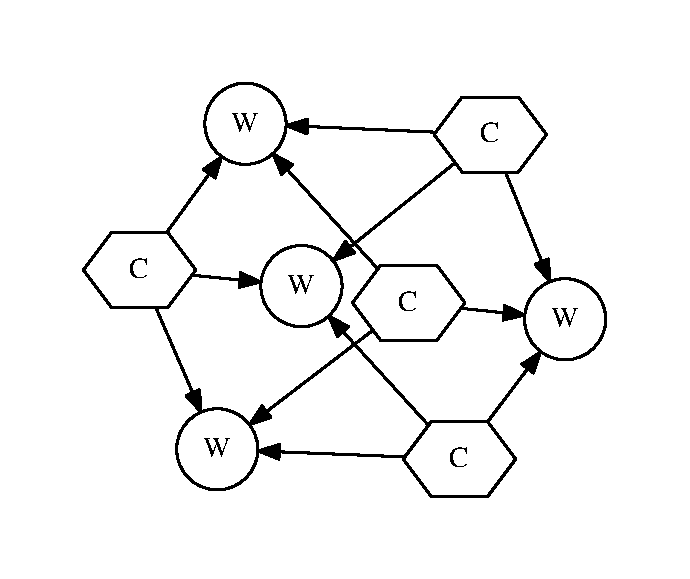
\includegraphics[width=\textwidth]{wcgraph}
  \end{textblock*}

  {

  \begin{itemize}
  \item Nodes connected by Edges
  \item Directed Acyclic Graphs (DAG)
    \begin{itemize}
    \item Edge directs from tail to head node, no loops
    \item If node has zero or one ``input edge'' $\Rightarrow$ ``tree''
    \end{itemize}
  \item Undirected Cyclic Graphs (meshes)
    \begin{itemize}
    \item Express connectivity with no direction, cycles allowed.
    \item Wires and Cells can form a duel-node type mesh
    \item Wire-Cell/Cell-Wire but not Wire-Wire/Cell-Cell
    \item Walk mesh to find any wire in a cell and vice versa, cell
      given three wires, connecting wires given a set of cells
    \end{itemize}
  \end{itemize}
}
  \begin{lstlisting}
    // WireCellMap.h
    typedef std::map<const Cell*, WireSelection> CellMap;
    typedef std::map<const Wire*, CellSelection> WireMap;
  \end{lstlisting}
\end{frame}

\end{document}

